%--------------------------------------------------------------------------------
% Type of Document / Start of Document / Portfolio
%--------------------------------------------------------------------------------
\documentclass[12pt]{article}
%--------------------------------------------------------------------------------
% Size & Headings for Paper
%--------------------------------------------------------------------------------
\usepackage[a4paper]{geometry}
\usepackage[myheadings]{fullpage}
%--------------------------------------------------------------------------------

%--------------------------------------------------------------------------------
\usepackage{fancyhdr}
\usepackage{lastpage}
%--------------------------------------------------------------------------------
% Positioning Etc
%--------------------------------------------------------------------------------
\usepackage{graphicx, wrapfig, subcaption, setspace, booktabs}
\usepackage{booktabs}
\usepackage{longtable}
\usepackage{float}
%--------------------------------------------------------------------------------
% Font
%--------------------------------------------------------------------------------
\usepackage[T1]{fontenc}
\usepackage[font=small, labelfont=bf]{caption}
\usepackage{fourier}
\usepackage[protrusion=true, expansion=true]{microtype}
%--------------------------------------------------------------------------------
% Language
%--------------------------------------------------------------------------------
\usepackage[english]{babel}
\usepackage{sectsty}
%%
%%
\newcommand{\HRule}[1]{\rule{\linewidth}{#1}}
\onehalfspacing
\setcounter{tocdepth}{5}
\setcounter{secnumdepth}{5}
%--------------------------------------------------------------------------------
% HEADER & FOOTER
%--------------------------------------------------------------------------------
\pagestyle{fancy}
\fancyhf{}
\setlength\headheight{15pt}
\fancyhead[L]{Student No. x19411076}
\fancyhead[R]{National College of Ireland}
\fancyfoot[R]{Page \thepage\ of \pageref{LastPage}}
%--------------------------------------------------------------------------------
% References & Style
%--------------------------------------------------------------------------------
\usepackage{natbib}
\setcitestyle{aysep={,}}
%--------------------------------------------------------------------------------
% Image and Table Settings
%--------------------------------------------------------------------------------
\usepackage{graphicx}
\graphicspath{{images/}}
\usepackage{multirow}
\usepackage{booktabs}
%%
%% Links - must be last package
\usepackage[pdftex,colorlinks=true,urlcolor=black,citecolor=black,anchorcolor=black,linkcolor=black,filecolor=black]{hyperref}
%--------------------------------------------------------------------------------
% Title Page
%--------------------------------------------------------------------------------
\begin{document}
%%
%%
\title{ \normalsize \textsc{Module: Computational Thinking}
		\\ [2.0cm]
		\HRule{0.5pt} \\
		\LARGE \textbf{\uppercase{CA1 - Learning Portfolio}}
		\HRule{2pt} \\ [0.5cm]
		\normalsize \today \vspace*{5\baselineskip}}
%--------------------------------------------------------------------------------
% Date of last update 
%--------------------------------------------------------------------------------
\date{\today}
%--------------------------------------------------------------------------------
% Personal Details of Author 
%--------------------------------------------------------------------------------
\author{
        Name: Renato Gusani \\
		Student No: x19411076 \\ 
		National College of Ireland \\
		Programme: BSc (Honours) in Data Science \\
		Year 1 - Semester 1 }
%--------------------------------------------------------------------------------
% Title
%--------------------------------------------------------------------------------
\maketitle
%--------------------------------------------------------------------------------
% Fresh Page
%--------------------------------------------------------------------------------
\newpage
%--------------------------------------------------------------------------------
% Section title formatting
\sectionfont{\scshape}
%-------------------------------------------------------------------------------

%-------------------------------------------------------------------------------
% BODY / Introduction / Learning Outcomes
%-------------------------------------------------------------------------------
%--------------------------------------------------------------------------------
% LO1 Create high quality academic, technical and scientific documents using appropriate tools and technologies 
%--------------------------------------------------------------------------------
%--------------------------------------------------------------------------------
% LO2 Implement appropriate referencing techniques for both written text and programming code 
%--------------------------------------------------------------------------------
%--------------------------------------------------------------------------------
% LO3 Compose both technical and non-technical questions in a manner which elicits the required response and information 
%--------------------------------------------------------------------------------
%--------------------------------------------------------------------------------
% LO4 Apply critical thinking, teamwork, communication and problem-solving skills when working as part of a team  
%--------------------------------------------------------------------------------
%--------------------------------------------------------------------------------
% LO5 Analyse personal learning needs and identify ways in which to resolve those needs in an autonomous fashion, seeking the support of, and providing support to peers where appropriate
%--------------------------------------------------------------------------------
\section*{Introduction}
\label{sec:intro}
In this Portfolio I will be demonstrating my capability to adequately reflect upon personal experiences towards situations such as in group assignments and solo assignments where i apply critical thinking, teamwork and communication problem-solving skills, to solve  assignments for semester 1 of year 1 in my course at National College of Ireland and create a high quality academic technical and scientific document using LaTeX in the Overleaf online editor as well actualising suitable referencing procedures for composed text.
I will then Compose both technical and non-technical questions in a way which evokes the required response and data and i will then Examine my individual learning needs and distinguish ways in which to resolve those needs in an autonomous way, looking for the help of, and giving back to peers where fitting.

%--------------------------------------------------------------------------------

%--------------------------------------------------------------------------------
% Assignment 1
%--------------------------------------------------------------------------------

\section{Assignment I}
\label{sec:assignment1}

%--------------------------------------------------------------------------------

%--------------------------------------------------------------------------------
% 1. Describe in both non-technical and technical terms the main problem proposed to be solved in the assignment and its main requirements; 
%--------------------------------------------------------------------------------

\begin{enumerate}
\item \textbf{\emph{Non-technical and technical description: }} The first assignment i have chose to reflect upon is from my Introduction to Data Science module, In this assignment i was tasked with to locate appropriate data sets for a fictitious study that meets a certain criteria and requirements, i had to prepare a short report entailing how and why the discovered data sources are relevant and accessible for the study. I also had to note key details of the data sources, application areas, and how they could contribute to a study design.

%--------------------------------------------------------------------------------

%--------------------------------------------------------------------------------
% 2. Briefly describe the main approaches proposed to solve the problem and provide the references to them; if applicable, provide a comparison of the different approaches
%--------------------------------------------------------------------------------

\item \textbf{\emph{The main approaches proposed to solve the assignment: }} The main approaches proposed to me and my class to complete this assignment was to first come up with a fictitious study that we are passionate about, it could be anything from movies to gaming to sports, 
then to identify at least two data sets that would complement each other (e.g., if i was intersted in sports one data set could be from an official outlet such as FIFA and another from social media users like twitter).
The data sets should be collected using different methods (e.g., scraping social media or user generated websites, surveys filled by people, automatic recording of user activities, etc.),
the data sets should also be correctly sized (depending on the topic of the study these could range in size from a few hundreds to thousands or even millions of instances).
%%
%%
\newpage
%% 
%% 

%--------------------------------------------------------------------------------

%--------------------------------------------------------------------------------
% 3. Justify descriptively the approach chosen to develop the assignment 
%--------------------------------------------------------------------------------

\item \textbf{\emph{The approach chosen to develop the assignment: }} The approach i had chosen to complete this assignment was to first read upon previous published IEEE reports that had been uploaded to our Moodle page by the Director such as \cite{arghir-nicolae_moldovann_cloud-based_2018} and \cite{arghir-nicolae_moldovann_vqamap_2016}, these IEEE reports were published by the Director himself as well as the alumni of National College of Ireland, in particular the students from the MSc in Data Analytics course. After i had thoroughly read through these papers i had a much better understanding of how to structure my assignment with the specific double column IEEE formatting.

%--------------------------------------------------------------------------------

%--------------------------------------------------------------------------------
% 4. Present a brief description of the solution implemented. In case it involves programming code, the commented code shall be released using a version control system
%--------------------------------------------------------------------------------

\item \textbf{\emph{Description of the solution implemented: }} The solution implemented into this assignment was to first read upon other published IEEE reports, after that i created an Introduction that summarized the objectives of my report and the process i followed to find my data sets that i used.
I then presented the Data with it's characteristics and structure, i did this by using tables to summarize the main key information of my data sets. I then had a Literature Review section where i had discussed other studies that used similar data sets to mine, i kept the discussion at a high-level as much as i could as at this point i lacked the prior knowledge to understand many of the details in the IEEE papers.
I also implemented a study design into my report which i had discussed how and why the found data was relevant and fit for the study, I also briefly discussed other areas i could have applied the data and how it would be combined and analysed to find out information, after this i ended my report with a total of 7 references.
Since i had found data set which was so big that is was sufficient enough to have my entire report written about it instead of having 2 data sets, i had only had to include one data set in my report. I have listed the data set used in the assignment in the below Table \ref{tab:my-table} on the next page.
\end{enumerate}
\newpage
%--------------------------------------------------------------------------------
% Example table of the Steam Dataset as used in Assignment 1
%--------------------------------------------------------------------------------
\begin{table}[]
\caption{Steam Dataset}
\label{tab:my-table}
\resizebox{\textwidth}{!}{%
\begin{tabular}{@{}llll@{}}
\toprule
\textbf{Data Table}      & \multicolumn{1}{c}{\textbf{Description}}                                                  & \textbf{Attributes}                                                                                                                                                         & \textbf{Data Table Obtained Through}                                                                    \\ \midrule
Achievement\_Percentages & \begin{tabular}[c]{@{}l@{}}achievement completion\\   for all steam products\end{tabular} & appid, Name, Percentage                                                                                                                                                     & \begin{tabular}[c]{@{}l@{}}{[}ISteamUserStats::GetGlobalAchievement\\ PercentagesForApp{]}\end{tabular} \\
App\_ID\_Info            & \begin{tabular}[c]{@{}l@{}}Information for each\\  steam product\end{tabular}             & \begin{tabular}[c]{@{}l@{}}appid, Title, Type, Price, Release\_Date, \\   Rating, Required\_Age, Is\_Multiplayer\end{tabular}                                               & emulating the REST API                                                                                  \\
Friends                  & \begin{tabular}[c]{@{}l@{}}List of friends of steam\\   users\end{tabular}                & \begin{tabular}[c]{@{}l@{}}steamid, appid, playtime\_2weeks, \\   playtime\_forever, dataretrived\end{tabular}                                                              & {[}ISteamUser::GetFriendList{]}.                                                                        \\
Games\_1                 & \begin{tabular}[c]{@{}l@{}}Game data during initial \\ steam network\end{tabular}         & \begin{tabular}[c]{@{}l@{}}steamid, appid, playtime\_2weeks, \\   playtime\_forever, dataretrived\end{tabular}                                                              & {[}IPlayerService::GetOwnedGames{]}                                                                     \\
Games\_2                 & \begin{tabular}[c]{@{}l@{}}Game data requested\\   after steam network\end{tabular}       & \begin{tabular}[c]{@{}l@{}}steamid, appid, playtime\_2weeks, \\   playtime\_forever, dataretrived\end{tabular}                                                              & {[}IPlayerService::GetOwnedGames{]}                                                                     \\
Games\_Daily             & \begin{tabular}[c]{@{}l@{}}gameplay data for five\\   consecutive days\end{tabular}       & \begin{tabular}[c]{@{}l@{}}steamid, appid, playtime\_2weeks, \\   playtime\_forever, dataretrived\end{tabular}                                                              & {[}IPlayerService::GetOwnedGames{]}                                                                     \\
Games\_Developers        & \begin{tabular}[c]{@{}l@{}}names of developers\\   of steam products\end{tabular}         & appid, Developer                                                                                                                                                            & emulating the REST API                                                                                  \\
Games\_Genres            & \begin{tabular}[c]{@{}l@{}}names of genres for each\\   product on steam\end{tabular}     & appid, Genre                                                                                                                                                                & emulating the REST API                                                                                  \\
Games\_Publishers        & \begin{tabular}[c]{@{}l@{}}names of publishers for\\   each steam product\end{tabular}    & appid, Publisher                                                                                                                                                            & emulating the REST API                                                                                  \\
Groups                   & \begin{tabular}[c]{@{}l@{}}list of all groups of each\\   user\end{tabular}               & steamid, groupid, dataretrieved                                                                                                                                             & steamcommunity.com XML data                                                                             \\
Player\_Summaries        & \begin{tabular}[c]{@{}l@{}}profile summary for each\\   steam user\end{tabular}           & \begin{tabular}[c]{@{}l@{}}steamid, lastlogoff, primaryclanid,\\ timecreated, gameid, gameserverip,\\ loccountrycode, locstatecode,\\ loccityid, dataretrieved\end{tabular} & {[}ISteamUser::GetPlayerSummaries{]}                                                                    \\ \bottomrule
\end{tabular}%
}
\end{table}
%%
%%
\newpage
%%
%%

%--------------------------------------------------------------------------------

%--------------------------------------------------------------------------------
% Assignment 2
%--------------------------------------------------------------------------------

\section{Assignment II}
\label{sec:assignment2}

%--------------------------------------------------------------------------------

%--------------------------------------------------------------------------------
% 1. Describe in both non-technical and technical terms the main problem proposed to be solved in the assignment and its main requirements; 
%--------------------------------------------------------------------------------

\begin{enumerate}
\item \textbf{\emph{Non-technical and technical description: }} The second assignment i have chosen to include in this portfolio is from my Problem Solving and Programming Concepts
module. In this assignment i was tasked with to develop an application within the \cite{noauthor_snap!_nodate} software. The application had to be an innovative game where a player plays against a computer. The application had to be a game show, for example: "Who wants to be a millionaire" "Deal or no deal" etc. The application chosen to be created should not be the same as any current game shows. I had the job of coming up with a new game show so it was important that my idea was unique.

%--------------------------------------------------------------------------------

%--------------------------------------------------------------------------------
% 2. Briefly describe the main approaches proposed to solve the problem and provide the references to them; if applicable, provide a comparison of the different approaches
%------------------------------------------------------------------

\item \textbf{\emph{The main approaches proposed to solve the assignment: }} The main approach proposed to me and my class to complete this assignment was to work individually, and to only start to develop the game in \textbf{SNAP} after thoroughly planning the application using Storyboards (Wire-frames), Psuedocode, IPO's, Flow chart and evidence of testing.
Another proposed approach was that we could have used an entirely different software to \textbf{SNAP} which was \textbf{Scratch}
These two programmes do not have a drastic difference therefore we were allowed to use this instead of \textbf{SNAP} since most of the class already knows how to use \textbf{Scratch}. The environment in both programmes was near to identical.

%--------------------------------------------------------------------------------

%--------------------------------------------------------------------------------
% 3. Justify descriptively the approach chosen to develop the assignment 
%--------------------------------------------------------------------------------

\item \textbf{\emph{The approach chosen to develop the assignment: }} The approach i had chosen to develop this assignment was solely dependent on the idea of \textbf{Predator} which is a 1987 American science fiction action film directed by John McTiernan and written by brothers Jim and John Thomas. It stars Arnold Schwarzenegger as the leader of an elite military rescue team on a mission to save hostages in guerrilla-held territory in Central America, i did not start of my assignment with wire frames first but instead i had started by going straight into using \textbf{SNAP.}

%--------------------------------------------------------------------------------

%--------------------------------------------------------------------------------
% 4. Present a brief description of the solution implemented. In case it involves programming code, the commented code shall be released using a version control system
%--------------------------------------------------------------------------------

\item \textbf{\emph{Description of the solution implemented: }} After messing around using the software i came up with the scenery as well as two characters. I made sure to include in my game at least 2 player's as well as IF conditions and a Loop, i added both player names with their score counter at the top of the screen and made sure the user interface was easy to follow and included sound effects as well as the iconic Predator background OST. After completing my game using SNAP i then created a Storyboard that showed how my game looks like, Psuedocode which was a text description of how my game would work, an IPO chart to show Inputs, Process and Outputs, a Flow chart that shows a detailed flow chart of how the application will work and lastly a test and results file which showed evidence of testing, in the below Figure \ref{fig:Predator} i have included the stage where my game is set in.
\end{enumerate}
%%
%% Figure of Snap Assignment 2
%%
\begin{figure}[!th]
  \centering
  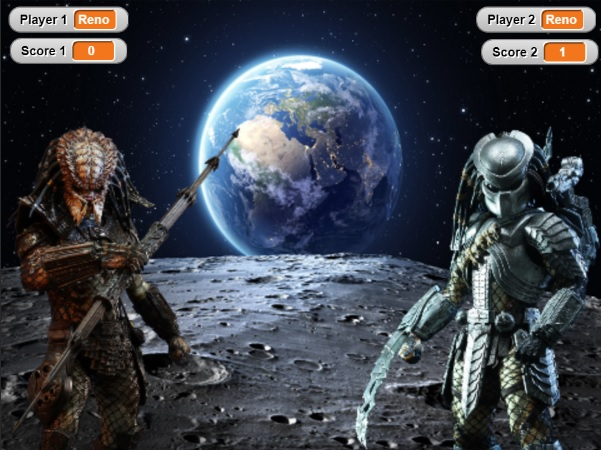
\includegraphics[width=4in]{Images/predator.jpg}
  \caption{Snap Stage.}
  \label{fig:Predator}
\end{figure}

%--------------------------------------------------------------------------------

%--------------------------------------------------------------------------------
% Assignment 3
%--------------------------------------------------------------------------------

\section{Assignment III}
\label{sec:assignment3}

%--------------------------------------------------------------------------------

%--------------------------------------------------------------------------------
% 1. Describe in both non-technical and technical terms the main problem proposed to be solved in the assignment and its main requirements; 
%--------------------------------------------------------------------------------

\begin{enumerate}
\item \textbf{\emph{Non-technical and technical description: }} The third and last assignment i have chosen to reflect upon and include in this portfolio is a group-based assignment from my Problem Solving and Design Principles module. This assignment is very similar to assignment  \ref{sec:assignment2}, except this time i had to work in a team of exactly 3 people, to design, create and test a new innovative game which could be played in The Cube. The game should comply with the rules of gameshow, it can be created any way i wanted and use any materials i want, the game could have been either a mental or physical game for one player. The Cube was a British game show that aired on ITV from 22 August 2009 to 8 August 2015 and was hosted by Phillip Schofield. The game is played by a single contestant within a transparent Perspex cube that measures 4 meters along each edge. The goal is to complete a series of seven games, each of which awards an increasing amount of prize money, before failing a total of nine times. Games are pre-selected for each individual contestant before the show to test their mental and physical faculties in various ways. 

%--------------------------------------------------------------------------------

%--------------------------------------------------------------------------------
% 2. Briefly describe the main approaches proposed to solve the problem and provide the references to them; if applicable, provide a comparison of the different approaches
%------------------------------------------------------------------
\item \textbf{\emph{The main approaches proposed to solve the assignment: }} This assignment had six deliverables similar to assignment \ref{sec:assignment2}, which were layed out in the following way, to first create a storyboard which illustrated the game idea, an IPO chart illustrating the Inputs, Process and Outputs of the game, a detailed psuedocode outline of the game, complete test plan documentation for the game, and lastly a video demo of the game being played and successfully completed.

%--------------------------------------------------------------------------------

%--------------------------------------------------------------------------------
% 3. Justify descriptively the approach chosen to develop the assignment 
%--------------------------------------------------------------------------------

\item \textbf{\emph{The approach chosen to develop the assignment: }} Since there was 3 of us doing this assignment, we had a discussion on dividing the workload evenly, we took into account that there was a total of six deliverables and therefore we would divide two deliverables to each of us. I personally took care of the Flow chart as well as the test and results for our game.

%--------------------------------------------------------------------------------

%--------------------------------------------------------------------------------
% 4. Present a brief description of the solution implemented. In case it involves programming code, the commented code shall be released using a version control system
%--------------------------------------------------------------------------------
% Fresh Page
%--------------------------------------------------------------------------------
\newpage
%--------------------------------------------------------------------------------

\item \textbf{\emph{Description of the solution implemented: }} The first thing me and my group needed to do was come up with a unique idea for a game, each of us had drawn up an example of multiple game ideas and we voted on which one we would do, which was colour-tiles. Colour tiles was a very simple physical game, which was basically matching 2 colours at a time in a sequence, our game had a timer as well as a score system, as well as a simplify option to make to the game reduce the amount of colours needing to be matched. After we had a concept of what we were going to do we went to work on our individual tasks and got feedback from the lecturer every time we had a completed task. Nearing the end it was noticeable one of us was slacking and not finishing at the pace the rest of us were, it came to the point where i personally had to take over a task and complete it with very little time to deadline. In the end me and my group came 2nd highest in the entire class and we also got a lot more experience in working in a group environment.
\end{enumerate}

%-------------------------------------------------------------------------------
% REFERENCES
%-------------------------------------------------------------------------------
\bibliographystyle{dcu}
\begin{center}
\nocite{*}
\bibliography{references}
\end{center}

%--------------------------------------------------------------------------------
% End of References
%--------------------------------------------------------------------------------

\end{document}

%--------------------------------------------------------------------------------
% End of Document / Portfolio
%--------------------------------------------------------------------------------